\documentclass{article}
\usepackage[utf8]{inputenc}
\usepackage{babel}
\usepackage{graphicx}
\usepackage[]{hyperref}
\usepackage[]{physics}
\usepackage[]{listings}
\usepackage{varioref}
\usepackage{float}
\usepackage{comment}
\usepackage[toc,page]{appendix}
\newcommand{\SL}{Schr\"{o}dinger }
\newcommand{\hbarm}{-\frac{\hbar^{2}}{2m}}
\newcommand{\ortwo}{\frac{1}{r^{2}}}
\newcommand{\ddr}{\frac{d}{dr}}
\newcommand{\ddrsq}{\frac{d^{2}}{dr^{2}}}
\newcommand{\ddrhosq}{\frac{d^{2}}{d\rho^{2}}}
\newcommand{\onehalf}{\frac{1}{2}}
\title{Using Jacobi's Rotation Algorithm to Solve the Two Electron \SL Equation}
\author{Kosar Nozari Mirarkolaei }
\date{September 2018}

\begin{document}

\maketitle

\section{Abstract}
\begin{abstract}
  In this project, I have implemented the Jacobi rotation algorithm to solve eigenvalue problem for one and two electrons in the Schr�dinger equation. I have found that the eigenvalues for the four lowest states to a very high precision. In the one electron case, they were found to be $\lambda_1 = 2.898$, $\lambda_2 = 6.8446$ , $\lambda_3 = 10.8016$ and $\lambda_4 = 14.7629$ compared to the analytical 3, 7 ,11 and 15 respectively.
		
There is also made a discussion of the speed of the algorithm compared to other methods, and in relation, pros and cons connected with the Jacobi method compared to one other method. The main idea here is that the Jacobi method is intrinsically  slow, but easy to parallelize. 
		
The source code for this project can be found at my github\footnote{\url{https://github.com/Kosarnm/FYS4150}}.  
\end{abstract}
\section{Introduction}
Eigenvalue problems are of great importance in the modern sciences. In this project, I will solve the radial part of the \SL equation for one and two electrons in a harmonic oscillator potential with and without repulsive Coulomb interaction using the Jacobi's rotation method for finding eigenvalues.

\section{Theory}
\subsection{The Buckling Beam Problem }
From the bucking beam problem we have the following equation:
$$\gamma\frac{d^2u(x)}{dx^2}=-Fu(x)$$
We also have the Dirichlet boundary condition which is $u(0)= 0$ and $u(L)= 0$ for x $\in [0,L]$.\\
In mechanical view $\textit{L}$ is the beam length and $\textit{F}$ is the force that apply at the (L,0) toward the origin and $\gamma$ is a constant that define by properties like rigidity of the beam.\\
Now we change the scale of the equation by defining dimensional variable $\rho$:
$$ \rho = \dfrac{x}{L}$$
Now by reordering the equation in $\rho \in [0,1]$ interval we have the following equation:
$$\frac{d^2 u(\rho)}{d\rho^2} = -\frac{FL^2}{R} u(\rho)=-\lambda u(\rho)$$
With discretizing the equation the problem change to the eigenvalue problem. Now we can use the expression for second derivative :
\begin{equation}
    u''=\frac{u(\rho+h) -2u(\rho) +u(\rho-h)}{h^2} +O(h^2),
    \label{eq:diffoperation}
\end{equation}
In the above equation $h$ is our step. And we also should define the maximum and minimum value for the variable $\rho$, $\rho_{min}$ and $\rho_{max}$. We consider $\rho_{min} = 0$ and $\rho_{max} = 1$. Now by considering $\rho_{min} = \rho_{0}$ and $\rho_{max} = \rho_{N}$ and with given number of mesh point $N$ we can define step length as:
$$ h=\frac{\rho_N-\rho_0 }{N}$$
And we can calculate $\rho$ at the different point of $i$ by using the following relation:
$$\rho_i= \rho_0 + ih \hspace{1cm} i=1,2,\dots , N$$
Then we rewrite the differential equation with $\rho_i$:
$$-\frac{u(\rho_i+h) -2u(\rho_i) +u(\rho_i-h)}{h^2}  = \lambda u(\rho_i)$$
This equation also can be written as:
$$-\frac{u_{i+1} -2u_i +u_{i-1} }{h^2}  = \lambda u_i$$
Now we can write this equation in the form of tridiagonal matrix for different value of $i$:
\begin{equation}
    \begin{bmatrix} d& a & 0   & 0    & \dots  &0     & 0 \\
                                a & d & a & 0    & \dots  &0     &0 \\
                                0   & a & d & a  &0       &\dots & 0\\
                                \dots  & \dots & \dots & \dots  &\dots      &\dots & \dots\\
                                0   & \dots & \dots & \dots  &a  &d & a\\
                                0   & \dots & \dots & \dots  &\dots       &a & d\end{bmatrix}
                                 \begin{bmatrix} u_1 \\ u_2 \\ u_3 \\ \dots \\ u_{N-2} \\ u_{N-1}\end{bmatrix} = \lambda \begin{bmatrix} u_1 \\ u_2 \\ u_3 \\ \dots \\ u_{N-2} \\ u_{N-1}\end{bmatrix}
\label{eq:matrixse}
\end{equation}

As we can see the boundary condition $u_0$ and $u_N$ are not included in the matrix. Now we have the diagonal element $d=\dfrac{-2}{h^2}$ and non diagonal elements $ a = \dfrac{1}{h^2}$
For finding analytical eigenpair for eigenvalue problem we can use following equation:
\begin{equation}
\lambda_j = d+2a\cos{(\frac{j\pi}{N+1})} \hspace{1cm} j=1,2,\dots N-1
\end{equation}
\subsection{Schr�dinger equation for one electron}Following equation shows the radial part of Schr�dinger equation for one electron. We start with solving this equation:
\begin{equation}
	\hbarm	(\ortwo \ddr r^{2} - \frac{l(l+1)}{r^{2}}) R(r) + V(r)R(r) = E R(r)
\end{equation}
In above equation $V(r) = \dfrac{1}{2}kr^2$ is harmonic oscillator potential and $k = m\omega^{2}$ and $E$ is the energy of harmonic oscillator in three dimension. $\omega$ is the oscillator frequency. Energies are calculated by the following equation for $n = 0,1,2..$ and $l = 0,1,2..$. $n$ and $l$ are energy quantum number and orbital momentum quantum number respectively. 
$$E_{nl} = \hbar \omega (2n+l+\frac{3}{2})$$
Then we assume that $R(r) = (1/r)u(r)$ and rewrite the equation 4:
\begin{equation}
	\hbarm \ddrsq u(r) + (V(r) + \frac{l(l+1)}{r^{2}}\hbarm)u(r) = Eu(r)
\end{equation}
The boundary condition for this equation are $u(0) = 0$ and $u(\infty) = 0$.\\
Now we define a dimensionless variable $\rho = (1/\alpha)r$ where $\alpha$ is a constant and then rewrite the equation:
\begin{equation}
	-\frac{\hbar^{2}}{2m\alpha^{2}} \ddrhosq u(\rho) + (V(\rho) + \frac{l(l+1)}{\rho^{2}}\frac{\hbar^{2}}{2m\alpha^{2}})u(\rho) = E u(\rho)
\end{equation}
In this project for easier calculation we set $l = 0$ and substitute $V(\rho) = \onehalf k\alpha^{2}\rho^{2}$ in equation (6):
\begin{equation}
	-\frac{\hbar^{2}}{2m\alpha^{2}} \ddrhosq u(\rho) + \onehalf k\alpha^{2} \rho^{2}u(\rho) = E u(\rho)
\end{equation}
Now we multiply the both side of equation(7) by $2m\alpha^{2} \rho^{2} /\hbar^{2}$ and define some constant as below:
$$\frac{mk}{\hbar^{2}}\alpha^{4} = 1 \hspace{1cm}\lambda = \frac{2m\alpha^{2}}{\hbar^{2}}E$$
Then we can rewrite the Schr�dinger equation as:
\begin{equation}
	-\ddrhosq u(\rho) + \rho^{2} u(\rho) = \lambda u({\rho})
\end{equation}
Just like the previous section we can solve this equation by discretizing the equation. First we define the minimum and maximum value for the $\rho$,$\rho_{min} = 0$ and $\rho_{max}$. Since we cannot set $\rho_{max} = \infty$ we can solve the problem for different value of $\rho_{max}$. By setting $\rho_{min} =\rho_0$ and $\rho_{max} = \rho_N$ and having the given number of mesh point $N$, the step length can define as:
$$ h = \dfrac{\rho_N - \rho_0}{N}$$
The value of $\rho$ for different value of $i$:
$$\rho_i= \rho_0 + ih \hspace{1cm} i=1,2,\dots , N$$
Now we can rewrite the Schr�dinger equation for value of $\rho_i$:
$$
-\frac{u(\rho_i+h) -2u(\rho_i) +u(\rho_i-h)}{h^2}+\rho_i^2u(\rho_i)  = \lambda u(\rho_i)$$
Or it can rewrite in more simple way:
$$-\frac{u_{i+1} -2u_i +u_{i-1}}{h^2}+\rho_i^2u_i=-\frac{u_{i+1} -2u_i +u_{i-1} }{h^2}+V_iu_i  = \lambda u_i$$
In the above equation $V_i = \rho_i^2$ is the harmonic oscillator potential.\\
We define the diagonal and non-diagonal matrix element as $d_{i} = \frac{2}{h^{2}} + V_{i}$ and $e_{i}= \frac{1}{h^{2}}$ respectively. Now by using these simplification the Schr�dinger equation can be writen as:
\begin{equation*}
  d_{i}u_{i}+e_{i-1}u_{i-1}+e_{i+1}u_{i+1} = \lambda u_{i}
\end{equation*}
Now we can write this equation as matrix eigenvalue problem:
\begin{equation}
    \begin{bmatrix} d_0& e_0 & 0   & 0    & \dots  &0     & 0 \\
                                e_1 & d_1 & e_1 & 0    & \dots  &0     &0 \\
                                0   & e_2 & d_2 & e_2  &0       &\dots & 0\\
                                \dots  & \dots & \dots & \dots  &\dots      &\dots & \dots\\
                                0   & \dots & \dots & \dots  &e_{N-1}  &d_{N-1} & e_{N-1}\\
                                0   & \dots & \dots & \dots  &\dots       & & d_N\end{bmatrix}
                                 \begin{bmatrix} u_0 \\ u_2 \\ u_3 \\ \dots \\ u_{N-1} \\ u_{N}\end{bmatrix} = \lambda \begin{bmatrix} u_0 \\ u_2 \\ u_3 \\ \dots \\ u_{N-1} \\ u_{N}\end{bmatrix}
\label{eq:matrixse}
\end{equation}
\subsection{Schr�dinger equation for two electron}
The Schr�dinger equation for one electron has been studied in the previous section and it had been modeled with following equation. $E^{(1)}$  is the energy for one electron only:
\begin{equation*}
  -\frac{\hbar^2}{2 m} \frac{d^2}{dr^2} u(r) 
       + \frac{1}{2}k r^2u(r)  = E^{(1)} u(r),
\end{equation*}
Now we want to study two electron in harmonic oscillator well using repulsive Coulomb interaction. For two electron with no repulsive Coulomb interaction the Schr�dinger equation can been written as:
\begin{equation*}
\left(  -\frac{\hbar^2}{2 m} \frac{d^2}{dr_1^2} -\frac{\hbar^2}{2 m} \frac{d^2}{dr_2^2}+ \frac{1}{2}k r_1^2+ \frac{1}{2}k r_2^2\right)u(r_1,r_2)  = E^{(2)} u(r_1,r_2) .
\end{equation*}
For solving this equation we introduced two new coordinate $\mathbf{r} = \mathbf{r}_1-\mathbf{r}_2$ the relative coordinate and $\mathbf{R} = 1/2(\mathbf{r}_1+\mathbf{r}_2)$ the center of mass coordinate. Then we rewrite the Schr�dinger equation as:
\begin{equation*}
\left(  -\frac{\hbar^2}{m} \frac{d^2}{dr^2} -\frac{\hbar^2}{4 m} \frac{d^2}{dR^2}+ \frac{1}{4} k r^2+  kR^2\right)u(r,R)  = E^{(2)} u(r,R).
\end{equation*}
Then we can dived the equation into two r-dependent and R-dependent equation. Then we define the repulsive Coulomb interaction between two electrons:

\begin{equation*}
V(r_1,r_2) = \frac{\beta e^2}{|\mathbf{r}_1-\mathbf{r}_2|}=\frac{\beta e^2}{r},
\end{equation*}

and by adding it to the r-dependent part of equation:
\begin{equation*}
\left(  -\frac{\hbar^2}{m} \frac{d^2}{dr^2}+ \frac{1}{4}k r^2+\frac{\beta e^2}{r}\right)\psi(r)  = E_r \psi(r).
\end{equation*}
This equation is similar to the equation for the one electron case, so here is we also introduce a dimensionless variable $\rho = r/\alpha$ and by repeating the same steps we have:
\begin{equation*}
  -\frac{d^2}{d\rho^2} \psi(\rho) 
       + \frac{1}{4}\frac{mk}{\hbar^2} \alpha^4\rho^2\psi(\rho)+\frac{m\alpha \beta e^2}{\rho\hbar^2}\psi(\rho)  = 
\frac{m\alpha^2}{\hbar^2}E_r \psi(\rho) .
\end{equation*}
For making this equation more like the one electron case we define new frequency $\omega_r$:
    \begin{equation*}
\omega_r^2=\frac{1}{4}\frac{mk}{\hbar^2} \alpha^4,
\end{equation*}
We also define some new constant as we did in previous section:

\begin{equation*}
\alpha = \frac{\hbar^2}{m\beta e^2} \hspace{1.5cm} \lambda = \frac{m\alpha^2}{\hbar^2}E
\end{equation*}
Now the Schr�dinger equation can be rewrite as:

\begin{equation}
  -\frac{d^2}{d\rho^2} \psi(\rho) + \omega_r^2\rho^2\psi(\rho) +\frac{1}{\rho} = \lambda \psi(\rho).
\end{equation}
The corresponding matrix form of this equation can be written as:
\begin{center}
\begin{equation}
{Au} =
\begin{bmatrix}
  \frac{2}{\hbar^{2}} + V_{1} & -\frac{1}{\hbar^{2}} & 0 & \cdots & \cdots & 0 \\
  -\frac{1}{\hbar^{2}} & \frac{2}{\hbar^{2}} + V_{2} &  -\frac{1}{\hbar^{2}} & 0 &\cdots & \cdots \\
  0 & -\frac{1}{\hbar^{2}} & \frac{2}{\hbar^{2}} + V_{3} & -\frac{1}{\hbar^{2}} & 0 & \cdots \\
  \vdots & \vdots & \vdots & \vdots & \vdots & \vdots \\
  0 & \cdots & \cdots & -\frac{1}{\hbar^{2}} & \frac{2}{\hbar^{2}} + V_{N-2} & -\frac{1}{\hbar^{2}} \\
  0 & \cdots & \cdots & \cdots & -\frac{1}{\hbar^{2}} & \frac{2}{\hbar^{2}} + V_{N-1}
\end{bmatrix}
\begin{bmatrix}
	u_{1} \\
	u_{2} \\
	\vdots \\
	\\
	\\
	u_{N-1}
\end{bmatrix}
=	\lambda
\begin{bmatrix}
	u_{1} \\
	u_{2} \\
	\vdots \\
	\\
	\\
	u_{N-1}
\end{bmatrix}
\end{equation}
\end{center}
\subsection{Jacobi eigenvalue algorithm}
Jacobi eigenvalue algorithm is an iterative method for calculation of the
eigenvalues and eigenvectors of a symmetric matrix:
\subsubsection{Givens rotation}A Givens rotation is represented by a matrix of the form:
\begin{equation}
G(i,j,\theta) = \begin{bmatrix}
1 & \hdots & 0 &\hdots & 0 & \hdots & 0 \\
    \vdots & \ddots & \vdots & {} & \vdots & {} & \vdots \\
    0 & \hdots & c &\hdots & -s & \hdots & 0 \\
    \vdots & {} & \vdots & \ddots & \vdots & {} & \vdots \\
    0 & \hdots & s &\hdots & c & \hdots & 0 \\
    \vdots & {} & \vdots & {} & \vdots & \ddots & \vdots \\
0 & \hdots & 0 &\hdots & 0 & \hdots & 1
\end{bmatrix}
\end{equation}
where $c = cos\theta$ , $s = sin\theta$  appear intersection of i th and j th rows and columns. That is the non zero
elements of Givens matrix is given by $g_{kk} = 1$ for $k \neq i,j$
$$g_{ii}= c$$
$$g_{jj} = -s$$
$$g_{ij} = s \hspace{0.5cm}\text{for} i>j$$
\subsubsection{Description of Jacobi algorithm}
$S' = G^{T} SG$ where $G $ be a Givens rotation matrix and $S$ be a symmetric
matrix then $S'$ is also a symmetric matrix. $S'$ has entries:
$$S'_{ij} = S'_{ji} = (c^{2}-s^2)S_{ij} + sc(S_{ii} - S_{jj})$$
$$S'_{ik} = S'_{ki} = cS_{ik} - sS_{jk} \hspace{1cm}\text{for} k\ne i,j$$
$$S'_{jk} = S'_{kj} = sS_{ik} + cS_{jk} \hspace{1cm}\text{for} k\ne i,j$$
$$S'_{ii} = c^2S_{ii}-2scS_{ij} + s^2S_{jj}    $$
$$S'_{jj} = s^2S_{ii}+2scS_{ij} + c^2S_{jj}    $$
where $c = cos\theta$, $s = sin\theta$, $G $ is orthogonal,$S$ and $S'$ have the same Frobenious norm , however we can choose $\theta$ so that $S'_{ij} = 0$, in which case $S'$ has a large sum of squares on the diagonal.
$$S'_{ij} = (cos2\theta)S_{ij} +\onehalf(sin2\theta)(S_{ii} - S_{jj})$$
Then we set above equation equal to zero:
$$tan2\theta = \dfrac{2S_{ij}}{S_{jj} - S_{ii}}$$
The Jacobi eigenvalue method repeatedly performs rotation until the matrix becomes almost diagonal. Then
the diagonal elements are approximations of the eigenvalues of $S$.
\subsection{Orthogonality Preservation}
Unity transformation preserve orthogonality. For proving this, first, we consider a basis of vector $v_i$
\begin{equation*}
\vb{v}_i = \begin{bmatrix}
v_{i_1} \\
\vdots \\
v_{i_n}
\end{bmatrix}
\end{equation*}
We assume that $v_i$ is orthogonal:
\begin{equation}
\vb{v}_j^T\vb{v}_i=\delta_{ij}.
\end{equation}
For unity transformation $\vb{w}_i = U\vb{v}_i$ we can write:
\begin{align}
\vb{w}_i^T\vb{w}_j &= (U\vb{v}_i)^T  U\vb{v}_i= \vb{v}_i^TU^T U\vb{v}_j = \vb{v}_i^T I \vb{v}_j \nonumber \\
&\rightarrow \vb{w}_i^T\vb{w}_j = \vb{v}_i^T\vb{v}_j = \delta_{ij},
\end{align}
It shows that both orthogonality and dot product has been preserved.This fact will be used further in this project.
\section{Implementation}
I have implemented the above methods in the python programming language.The the values for the potential in both cases are known at $i=0$ and $i=n$, namely $V_0=0$ and $V_n=0$. To create the matrix in equation (2), we therefore only need values for $\rho_i$ for $i=1,2,...,n-1$, which are plugged into the diagonal elements $d_i$. 
\begin{lstlisting}[caption=Jacobi algorithm]
def jacobi_method(A, R, n):
    for i in range(0,n):
        for j in range(0,n):
            if i==j:
                R[i][j] = 1.0
            else:
                R[i][j] = 0.0
    tol = 1.0e-10
    max_iteration = n**4
    iteration = 0
    max_offdiagonal,l,k = maxoff(A,n)
    while abs(max_offdiagonal) > tol and iteration < max_iteration :
        max_offdiagonal,l,k = maxoff(A,n)
        rotate(A,R,k,l,n)
        iteration +=1
    print('number of iteration: ' ,iteration , '\n')
			\end{lstlisting}
where the function \texttt{rotate} follows the rotation algorithm presented in section (2.4.2). The function \texttt{maxoff} finds and returns the largest element in the current matrix $\A$, also changing the values of $k$ and $l$ so that these refer to the largest element in $\A$.
\section{Results and Discussion}
\subsection{Setting up a code for tridiagonal Toeplitz matrix}
Using the code which was describe in the previous section, We define $\tan\theta = t = \dfrac{s}{c}$, $\sin\theta = s$ and $\cos\theta = c$.
\begin{equation*}\cot 2\theta=\tau = \frac{a_{ll}-a_{kk}}{2a_{kl}}.
\end{equation*}
Now we can define the angel of $\theta$ in order that the non-diagonal element of the matrix become zero.
Given the facts $\cot 2\theta=1/2(\cot \theta-\tan\theta)$ and $\cot\theta = \dfrac{1}{\tan\theta}$ and since $\tan\theta = t$:
\begin{equation*}\tau = 1/2(\dfrac{1}{t}- t)\hspace{0.5cm}\Rightarrow\hspace{0.5cm} t^2+2\tau t-1= 0
\end{equation*}
Solving above equation:
\begin{equation*}
  t = -\tau \pm \sqrt{1+\tau^2},
\end{equation*}
Now the $c$ and $s$ obtain easily:
\begin{equation*}
   c = \frac{1}{\sqrt{1+t^2}},\hspace{1cm} s=tc
\end{equation*}
Taable~\vref{tab:first} shows numerical and analytical
eigenvalues for N = 10:

\begin{table}[!hb]
				\centering
				\caption{The accuracy of $\lambda$ increases as the density of grid points increases, here represented by decreasing values of $\rho_\mathrm{max}$. $n=200$.}
				\label{table: eigenvalues and rho_max}
				\begin{tabular}{|c|c|}
					\hline
					$Analytical$	&	$numerican3$	\\
					\hline
-0.512890         & -0.51289         \\\hline
3.64507           & 3.64507          \\\hline
0.16574           & 0.16574          \\\hline
2.88523           & 2.88523          \\\hline
2.20157           & 2.20157          \\\hline
1.45647           & 1.45647          \\\hline
1.78628           & 1.78628          \\ \hline
1.92128           & 1.92128          \\ \hline
1.84952           & 1.45647          \\ \hline
1.13062           & 1.13062          \\ \hline
					\hline
				\end{tabular}
			\end{table}
\subsection{Unit Test}
In this section I implemented two unit test for the code. The $maxoff$ function has been checked whether it return the correct value for the maximum off-diagonal element for a given simple test matrix. The function returns the expected value so it shows that this part of program works properly. The eigenvalues of a matrix do not change after rotations. We should get the same eigenvalues for both the original matrix and the matrix after some rotations. Get the same eigenvalues for matrix before and after rotation shows that our $rotate$ function works as expected.


\begin{figure}
    \centering
    \begin{subfigure}
    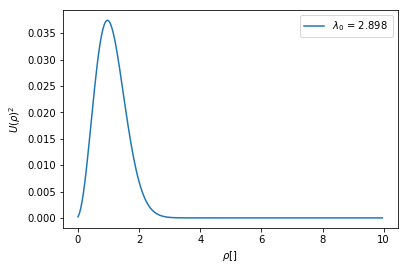
\includegraphics[width=8cm, height=5cm]{lambda_3.png}
    \end{subfigure}%
    \begin{subfigure}
    \centering
    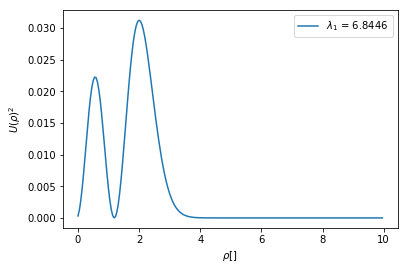
\includegraphics[width=8cm, height=5cm]{lambda_7.png}
    \end{subfigure}%
    
    \begin{subfigure}
    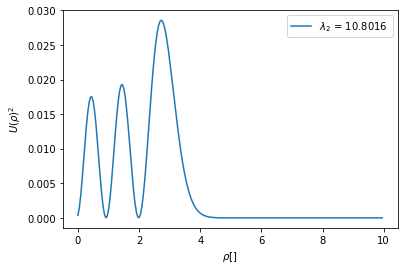
\includegraphics[width=8cm, height=5cm]{lambda_11.png}
    \end{subfigure}
    \caption{Probability distribution of the eigenstates for one electron in the harmonic oscillator potential. As we can see, the eigenvalues are not completely equal to the theoretical results. In this example, $n=220$ grid points and $\rho_\mathrm{max}=10$ were used.}
    \label{fig:my_label}
\end{figure}


\subsection{ Quantum dots in three dimensions, one electron}
In this section I use Schr�dinger equation for one electron (2.2) for solving the eigenvalue problem.Here we can use same code which we develop using the Jacobi�s rotation algorithm. But we need to add the harmonic oscillator potential $V_i = \rho^2$ to the diagonal element of the matrix.Figur 1 shows the eigenstates of the electron plotted as a probability distribution as a function of $\rho$. The respective eigenvalues are indicated, and resemble those found theoretically, building confidence in the reliability of the program. The value of $\rho_\mathrm{max}$ should, ideally, be $\infty$, but as Figure 1 shows, the probability of finding the electron outside of $\rho_\mathrm{max}\approx 5$ is almost, or equal to, zero for the four lowest eigenstates. One can therefore increase the accuracy by setting $\rho_\mathrm{max}$ lower, without needing to increase the number of grid points. Table 2 shows such a relation. Note that decreasing $\rho_\mathrm{max}$ into an area where there is a larger than zero probability of finding the electron ($\rho_\mathrm{max}<\sim 4$), has the effect of decreasing the accuracy.\\
By the method of trial and error, it was found that $n=220$ is enough to get the three first eigenvalues stable to four leading digits.\\
It is also of interest to find the number of transformations needed as a function of the number of grid points. The number of iterations needed goes like $\sim O(n^2)$.

\begin{table}[]
\centering
\begin{tabular}{|l|l|l|l|l|}

\caption{The accuracy of $\lambda$ increases as the density of grid points increases, here represented by decreasing values of $\rho_\mathrm{max}$. $n=220$.}
\hline
$\rho_max$ & $\lambda_0$ & $\lambda_1$ & $\lambda_2$ & $\lambda_3$ \\ \hline
10         & 2.8984      & 6.8446      & 10.8016     & 14.7629     \\ \hline
8          & 2.919       & 6.86        & 10.842      & 14.812      \\ \hline
6          & 2.939       & 6.907       & 10.882      & 14.861      \\ \hline
4          & 2.959       & 6.941       & 10.997      & 15.442      \\ \hline
\end{tabular}
\end{table}{Tabel 2}

\subsection{Quantum dots in three dimensions, two electron}
For solving eigenvalue problem ,I use Schr�dinger equation for two electrons. The algorithm is same as the one we had for the tridiagonal Toeplitz matrix. However, we need to add potential  $\omega_r^2\rho^2+1/\rho$ to the diagonal elements.\\
For the case of two electrons, we are interested in the wavefunction for the ground state (lowest eigenvalue) for four different values of the oscillator "frequency" $\omega_r$. The results are shown in Figure 2. As the plot show, the oscillator frequency greatly influences the probability distribution of the position of the center of mass for the electron pair, higher frequencies leading to a narrower distribution, much closer to the origin. One other thing to note is that higher frequency leads to larger eigenvalue. This makes direct sense, as the eigenvalues $\lambda\propto E$, and higher frequencies give higher energies.

\begin{figure*}[t!]
    \centering
    \begin{subfigure}
        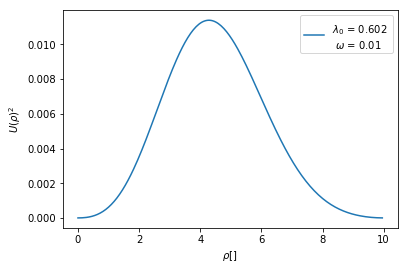
\includegraphics[width=8cm, height=5cm]{omega_001.png}
    \end{subfigure}
    \begin{subfigure}
        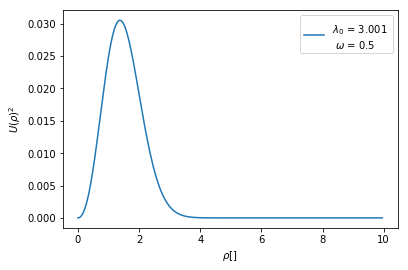
\includegraphics[width=8cm, height=5cm]{omega05.png}
    \end{subfigure}
    
    \begin{subfigure}
        \centering
        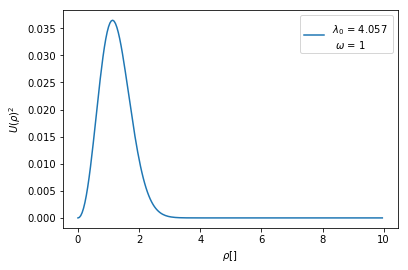
\includegraphics[width=8cm, height=5cm]{omega1.png}
    \end{subfigure}
    \caption{Plot of the probability distributions for two electrons with four different oscillator "frequencies" $\omega_r$.} 
    \label{fig:my_label}
\end{figure*}{figure 2}
\end{document}
\section{Conclusion}
The Jacobi method is a very slow method of finding eigenvalues compared to the method embedded in the python \texttt{numpy} library. On average, it is needed around $O(n^2)$ Jacobi rotations to find the eigenvalues of an $n\times n$ matrix, each rotation using around 30-40$n$ FLOPS, leading to $\sim O(n^3)$ FLOPS. 
We have seen that both methods reaches convergence for the three lowest eigenvalues relatively quickly at $n\approx 200$. A good reason to use the Jacobi method that is easily parallelizable, so for systems where a relatively small number of grid points $n$ is sufficient, the Jacobi method may be the preferred method.
		
	
